{\small

\section{О приложении алгебры к геометрии}

\paragraph{}\label{1938/209}
\so{Задача}.
\emph{Данный отрезок разделить в среднем и крайнем отношении.}

Эту задачу надо понимать так:
разделить данный отрезок на такие две части, чтобы б\'{о}льшая из них была средней пропорциональной между всей линией и меньшей её частью.

Задача будет решена, если мы найдём одну из двух частей, на которые требуется разделить данный отрезок.
Будем находить б\'{о}льшую часть, то есть ту, которая должна быть \so{средней пропорциональной} между всем отрезком и меньшей его частью.
Предположим сначала, что речь идёт не о построении этой части, а только о \so{вычислении} её длины.
Тогда задача решается \so{алгебраически} так:
если длину данного отрезка обозначим $a$, а длину б\'{о}льшей части $x$, то длина другой части будет равна $a-x$ и, согласно требованию задачи, мы будем иметь пропорцию:
\[\frac ax=\frac x{(a-x)}.\]
откуда
\[x^2=a(a-x),
\quad\text{или}\quad
x^2+ax-a^2=0.\]
Решив это квадратное уравнение, находим:
\[
x_1=-\frac a2 + \sqrt{\left(\frac a2\right)^2+a^2};
\quad
x_2=-\frac a2 - \sqrt{\left(\frac a2\right)^2+a^2}.
\]
Отбросив второе решение, как отрицательное, возьмём только первое положительное решение, которое удобнее представить так:
\begin{align*}
x_1&= \sqrt{\left(\frac a2\right)^2+a^2}-\frac a2 =
\\
&= \sqrt{\frac {a^2}4+a^2}-\frac a2 =
\\
&= \sqrt{\frac {5a^2}4}-\frac a2 =
\\
&= \frac a2\sqrt{5}-\frac a2 =
\\
&= \frac {a(\sqrt{5}-1)}2 \approx
\\
&\approx a\cdot 0{,}61803.
\end{align*}
Таким образом, задача всегда имеет решение и притом только одно.

Если бы нам удалось построить такой отрезок, длина которого выражается найденной выше формулой, то нанеся этот отрезок на данный отрезок, мы разделили бы его в среднем и крайнем отношении.
Итак, вопрос сводится к построению найденной формулы.
Построить эту формулу всего удобнее, если мы её возьмём в том виде, в каком она была до упрощения, то есть возьмём:
\[x_1= \sqrt{\left(\frac a2\right)^2+a^2}-\frac a2.\]

\begin{wrapfigure}{o}{45mm}
\centering
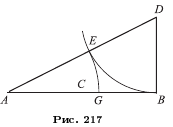
\includegraphics{mppics/ris-217}
\caption{}\label{1938/ris-217}
\end{wrapfigure}

\noindent
Выражение $\sqrt{(\frac a2)^2+a^2}$ представляет собой длину гипотенузы такого прямоугольного треугольника, у которого один катет равен $a$, а другой $\frac a2$.
Построив такой треугольник, мы найдём отрезок, выражаемый формулой $\sqrt{(\frac a2)^2+a^2}$.
Чтобы получить затем отрезок $x_1$, достаточно из гипотенузы построенного треугольника вычесть $\frac a2$.
Таким образом, построение можно выполнить так:

Делим (рис.~\ref{1938/ris-217}) данный отрезок $AB=a$ пополам в точке $C$.
Из конца $B$ восстанавливаем перпендикуляр и откладываем на нём $BD = BC$.
Соединив $A$ с $D$ прямой, получим прямоугольный $\triangle ABD$, у которого один катет $AB=a$, а другой катет $BD=\frac a2$.
Следовательно, его гипотенуза $AD$ равна $\sqrt{(\frac a2)^2+a^2}$.
Чтобы вычесть из гипотенузы длину $\frac a2$, опишем дугу радиусом $BD=\frac a2$ с центром в точке $D$.
Тогда отрезок $AE$ будет равен $\sqrt{(\frac a2)^2+a^2}-\frac a2$, 
то есть будет равен $x_1$.
Отложив $AE$ на $AB$ (от $A$ до $G$), получим точку $G$, в которой отрезок $AB$ делится в среднем и крайнем отношении%
\footnote{Деление отрезка в среднем и крайнем отношении известно под названием \rindex{золотое сечение}\textbf{золотого сечения}.}%
.

{\small
\smallskip
\so{Замечание}.
Деление отрезка в среднем и крайнем отношении нужно в геометрии для построения правильного 10-угольника, вписанного в данный круг.
}

\paragraph{Алгебраический способ решения геометрических задач.}\label{1938/210}
Мы решили предложенную задачу путём приложения алгебры к геометрии.
Этот приём состоит в следующем:
сперва определяют, какой отрезок прямой нужно отыскать, чтобы решить задачу.
Затем, обозначив длины данных отрезков буквами $a, b, c,\dots$, а искомого буквой $x$, составляют из условий задачи и известных теорем уравнение, связывающее длину искомого отрезка с длинами данных, и полученное уравнение решают по правилам алгебры.
Найденную формулу исследуют, то есть определяют, при всяких ли данных $a, b, c,\dots$ эта формула определяет решение или только при некоторых и получается ли одно решение или несколько.
Затем строят формулу, то есть находят построением такой отрезок, длина которого выражается этой формулой.

Таким образом, алгебраический приём решения геометрических задач состоит в общем из следующих четырёх частей:
1) составление уравнения;
2) решение его;
3) исследование полученной формулы и 4) построение её.

{\sloppy 
Иногда задача сводится к отысканию нескольких отрезков.
Тогда, обозначив их длины буквами $x,y,\dots$, стремятся составить столько уравнений, сколько неизвестных.

}

\paragraph{Построение простейших формул.}\label{1938/211}
{\sloppy 
Укажем простейшие формулы, которые можно построить посредством циркуля и линейки;
при этом будем предполагать, что буквы $a$, $b$, $c,\dots$
означают длины данных отрезков, а $x$ — длину искомого.
Не останавливаясь на таких формулах:
\[x=a+b+c,
 \quad
 x=a-b,
 \quad
 x=2\cdot a,\ 3\cdot a,\dots,
\]
построение которых выполняется весьма просто, перейдём к более сложным:

}

1) Формулы $x=\frac a2, \frac a3,\dots$ и~т.~д. строятся посредством деления отрезка $a$ на равные части, затем, если нужно, повторением одной части слагаемых $2, 3,\dots$ и так далее раз.

{\sloppy

2) Формула $x=\frac{ab}c$ выражает \so{четвёртую пропорциональную} к отрезкам $c$, $a$ и $b$.
Действительно, из этого равенства выводим:
\[c\cdot x=a\cdot b,
\quad\text{откуда}\quad
\frac ca=\frac bx.\]

}

Следовательно, $x$ найдётся способом, указанным нами для построения четвёртой пропорциональной (§~\ref{1938/185}).

3) Формула $x=\frac{a^2}b$ выражает четвёртую пропорциональную к отрезкам $b$, $a$ и $a$, или, как говорят, \so{третью пропорциональную} к отрезкам $b$ и $a$.
Действительно, из данного равенства выводим:
\[b\cdot x=a^2,
\quad\text{откуда}\quad
\frac ba=\frac ax.\]
Следовательно, $x$ найдётся тем же способом, каким отыскивается четвёртая пропорциональная (только отрезок $a$ придётся откладывать два раза).

{\sloppy

4) Формула $x=\sqrt{a\cdot b}$ выражает \so{среднюю пропорциональную} между $a$ и $b$.
Действительно, из неё выводим:
\[x^2=a\cdot b,
\quad\text{откуда}\quad\frac ax=\frac xb.\]

}

Следовательно, $x$ найдётся способом, указанным раньше для построения средней пропорциональной (§~\ref{1938/190}).

5) Формула $x=\sqrt{a^2+b^2}$ выражает \so{гипотенузу} прямоугольного треугольника с катетами $a$ и $b$.


6) Формула $x=\sqrt{a^2-b^2}$ представляет катет прямоугольного треугольника с гипотенузой $a$ и другим катетом $b$.

Построение всего удобнее выполнить так, как указано в §~\ref{1938/126}.
Указанные формулы можно считать основными.
При помощи их строятся более сложные формулы.
Например:

7) $x=a\sqrt{\frac23}$.
Подведя $a$ под знак радикала, получим:
\[x=\sqrt{\tfrac23a^2}=\sqrt{a\cdot\tfrac23a}.\]
Отсюда видно, что $x$ есть средняя пропорциональная между отрезками $a$ и~$\tfrac23a$.

8) $x=\sqrt{a^2 + b^2 - c^2 + d^2}$.
Положим, что  $a^2+b^2=k^2$.
Тогда $k$ найдётся как гипотенуза прямоугольного треугольника с известными катетами $a$ и $b$.
Построив $k$, положим, что $k^2+d^2=\ell^2$.
Тогда $\ell$ найдётся как гипотенуза прямоугольного треугольника с катетами $k$ и $d$.
Построив $\ell$, будем иметь $x=\sqrt{\ell^2-c^2}$.
Следовательно, $x$ есть катет такого треугольника, у которого гипотенуза $\ell$, а другой катет~$c$.

Ограничимся этими примерами.
Заметим, что подробное рассмотрение способов построения алгебраических формул приводит к следующему важному выводу.

\emph{При помощи линейки и циркуля возможно строить только такие алгебраические выражения, которые могут быть получены из длин известных отрезков с помощью конечного числа арифметических операций \emph{(то есть сложения, вычитания, умножения и деления)} 
и извлечения квадратных корней}.

}

{\small

\subsection*{Упражнения}

\begin{center}
\so{Доказать теоремы}
\end{center}

\begin{enumerate}[noitemsep]

\item
Прямая, проведённая через середины оснований трапеции, проходит через точку пересечения продолжений боковых сторон и через точку пересечения диагоналей.

\item
Если в треугольнике из вершины угла, лежащего между неравными сторонами, проведены биссектриса и медиана, то первая меньше второй.

\item
Если два круга касаются извне, то часть внешней общей касательной, ограниченная точками касания, есть средняя пропорциональная между диаметрами кругов.

\item
Если на сторонах угла отложим от вершины пропорциональные отрезки, то прямые, соединяющие соответственные концы их, параллельны.

\item
Если в прямоугольный треугольник $ABC$ вписать квадрат $DEFG$ так, чтобы сторона $DE$ лежала на гипотенузе $BC$, то эта сторона есть средняя пропорциональная между отрезками гипотенузы $BD$ и $EC$ (точки на гипотенузе следуют в порядке $B$, $D$, $E$, $C$).

\item
Если два отрезка $AB$ и $CD$ пересекаются в точке $E$ так, что $BE\cdot  EA\z=EC\cdot  ED$, то точки $A$, $B$, $C$ и $D$ лежат на одной окружности (теорема, обратная изложенной в §~\ref{1938/200}).

\item
Дана окружность с центом $O$ и две точки $A$ и $B$.
Через эти точки проведено несколько окружностей, пересекающих окружность $O$ или касающихся её.
Доказать, что все хорды, соединяющие точки пересечения каждой из этих трёх окружностей с окружностью $O$, а также и общие касательные либо параллельны, либо сходятся (при продолжении) в одной точке, лежащей на прямой $AB$. 

\item
Основываясь на свойстве, изложенном в предыдущей задаче, вывести способ построения такой окружности, которая проходит через две данные точки $A$ и $B$ и касается данной окружности.

\item
Даны два каких-нибудь круга на плоскости.
Если два радиуса этих кругов движутся, оставаясь постоянно параллельными, то прямая, проходящая через концы их, пересекает линию центров всегда в одной и той же точке (в \so{центре подобия} двух кругов).

\item
Медиана треугольника делит пополам все прямые, проведённые внутри треугольника параллельно той стороне, относительно которой взята медиана.

\item
Даны три прямые, исходящие из одной точки.
Если по одной из них движется какая-нибудь точка, то расстояния от неё до двух других прямых сохраняют всегда одно и то же отношение.

\item
Если две окружности концентрические, то сумма квадратов расстояний от всякой точки одной из них до концов какого угодно диаметра другой есть величина постоянная (§~\ref{1938/197}).

\item
Если соединим прямыми основания трёх высот какого-нибудь треугольника, то образовавшиеся при этом три треугольника у вершин данного подобны ему.

Вывести отсюда, что для треугольника, имеющего сторонами прямые, соединяющие основания высот данного треугольника, эти высоты служат биссектрисами.

\item
{\sloppy 
Диаметр $AB$ данной окружности продолжен за точку $B$.
Через какую-нибудь точку $C$ этого продолжения проведена прямая $CD\z\perp AB$.
Если произвольную точку $M$ этого перпендикуляра соединим с $A$, (обозначив через $A_1$ вторую точку пересечения с окружностью этой прямой), то произведение $AM\cdot  AA_1$ есть величина постоянная для всякой точки $M$.

}

\end{enumerate}

\begin{center}
\so{Найти геометрические места}
\end{center}

\begin{enumerate}[resume,noitemsep]

\item
Середин всех хорд, проходящих через данную точку окружности.

\item
Точек, делящих в одном и том же отношении $m:n$ все хорды, проходящие через данную точку окружности.

\item \label{1938/upr-3-17}
Точек, расстояние от которых до сторон данного угла имеет одно и то же отношение $m:n$.

\item
Точек, для которых сумма квадратов расстояний до двух данных точек есть величина постоянная (§~\ref{1938/197}).

\item
Точек, для которых разность квадратов расстояний до двух данных точек есть величина постоянная.

\item
Точек, делящих в данном отношении $m:n$ все прямые, соединяющие точки окружности с данной точкой $O$ (лежащей вне или внутри круга).

\end{enumerate}

\begin{center}
\so{Задачи на построение}
\end{center}

\begin{enumerate}[resume,noitemsep]

\item
Через точку, данную внутри или вне угла, провести прямую так, чтобы отрезки её, заключённые между этой точкой и сторонами угла, имели данное отношение $m:n$.

\item
Найти в треугольнике такую точку, чтобы перпендикуляры, опущенные из неё на стороны треугольника, находились в данном отношении $m:n:p$ (смотри упражнение \ref{1938/upr-3-17}).

\item
Построить треугольник по углу, одной из сторон, прилежащих к нему, по отношению этой стороны к третьей стороне (сколько решений?).

\item
То же — по углу при вершине, основанию и отношению его к одной из боковых сторон.

\item
То же — по высоте, углу при вершине и отношению отрезков основания.

\item
То же — по углу при вершине, основанию и данной на основании точке, через которую проходит биссектриса угла при вершине.

\item
То же — по двум углам и сумме или разности основания с высотой.

\item
Построить равнобедренный треугольник по углу при вершине и сумме основания с высотой.

\item
На бесконечной прямой $MN$ даны две точки $A$ и $B$.
Найти на этой прямой третью точку $C$, чтобы $CA:CB=m:n$, где $m$ и $n$ — данные отрезки или данные числа (если $m\ne n$, то таких точек существует две:
одна между $A$ и $B$, другая вне отрезка $AB$).

\item
Вписать в данный круг треугольник, у которого даны:
основание и отношение двух сторон.

\item
Вписать в данный круг треугольник, у которого даны:
основание и медиана к одной из неизвестных сторон. 

\item
Вписать квадрат в данный сегмент так, чтобы одна его сторона лежала на хорде, а вершины противолежащих углов — на дуге.

\smallskip
\so{Указание}.
Задачи решаются методом подобия (§~\ref{1938/181}).

\item
Вписать квадрат в данный треугольник так, чтобы одна сторона его лежала на основании треугольника, а вершины противолежащих углов — на боковых сторонах треугольника.

\item
В данный треугольник вписать прямоугольник (смотри предыдущую задачу), у которого стороны относились бы как $m:n$.

\item
Около данного квадрата описать треугольник, подобный данному треугольнику.

\item
Дана окружность и на ней две точки $A$ и $B$.
Найти на этой окружности третью точку $C$, чтобы расстояния от неё до $A$ и $B$ находились в данном отношении.

\item %%%%overfull
Построить треугольник по двум сторонам и биссектрисе угла между ними (смотри рис.~\ref{1938/ris-196};
сначала находим прямую $CE$ из пропорции $CE:BD=AE:AB$, затем строим $\triangle BCE$ и~т.~д.).

\item
Построить отрезок $x$, который относился бы к данному отрезку $m$ как $a^2:b^2$ ($a$ и $b$ — данные отрезки).

\item
Найти вне данного круга такую точку, чтобы касательная, проведённая из неё к этой окружности, была вдвое менее секущей, проведённой из той же точки через центр (приложением алгебры к геометрии).

\item
Через данную вне круга точку провести такую секущую, которая разделилась бы этой окружностью в данном отношении (приложением алгебры к геометрии).

\item
Построить треугольник по трём его высотам $h_1$, $h_2$, $h_3$

\smallskip
{\sloppy 
\so{Решение}.
Предварительно из подобия прямоугольных треугольников надо доказать, что высоты \so{обратно пропорциональны} соответствующим сторонам.
Если стороны, на которые опущены высоты $h_1$, $h_2$, $h_3$ обозначим соответственно через $x_1$, $x_2$, $x_3$, то
\[x_1:x_2=h_2:h_1,\]
\[x_2:x_3=h_3:h_2=1:\frac{h_2}{h_3}=h_1:\frac{h_1h_2}{h_3}\]
откуда 
\[x_1:x_2:x_3=h_2:h_1:\frac{h_1h_2}{h_3}\]
Выражение $\frac{h_1h_2}{h_3}$ есть четвёртая пропорциональная к $h_1$, $h_2$ и $h_3$.
Построив её (пусть это будет $k$), мы будем иметь три отрезка:
$h_2$, $h_1$ и $k$, которым искомые стороны пропорциональны;
значит, треугольник, имеющий эти отрезки сторонами, подобен искомому, и потому вопрос сводится к построению такого треугольника, который, будучи подобен данному, имел бы данную высоту.
Задача не имеет решения, если по трём прямым $h_1$, $h_2$ и $k$ нельзя построить треугольник.

}

\item
Построить отрезки, выражаемые формулами: 
\[1)\ x=\frac{abc}{de}=\frac{ab}{d}\cdot \frac{c}{e}\]
(придётся два раза построить четвёртую пропорциональную).
\[2)\ x=\sqrt{a^2+bc}.\]
(предварительно построить отрезоки $k=\sqrt{bc}$ и $x=\sqrt{a^2+k^2}$).

\end{enumerate}

\begin{center}
\so{Задачи на вычисление}
\end{center}

\begin{enumerate}[resume,noitemsep]

\item
По данному основанию $a$ и высоте $h$ остроугольного треугольника вычислить сторону $x$ квадрата, вписанного в этот треугольник так, что одна сторона квадрата лежит на основании треугольника, а две вершины квадрата — на боковых сторонах треугольника.

\item
Стороны треугольника имеют длины 10, 12 и 17 м.
Вычислить отрезки стороны, равной 17 м, на которые она делится биссектрисой противолежащего угла.

\item
Перпендикуляр, опущенный из вершины прямого угла на гипотенузу, делит её на два отрезка $m$ и $n$.
Вычислить катеты.

\smallskip
\so{Указание}.
Продолжив $AD$ на расстояние $DE=AD$ и соединив точку $E$ с $B$ и $C$, получим параллелограмм, к которому применим теорему §~\ref{1938/197}.

\item
В $\triangle ABC$ стороны равны:
$AB$ = 7, $BC$ = 15 и $AC$ = 10.
Определить, какого вида угол $A$, и вычислить высоту, опущенную из вершины $B$.

\item
Из точки вне круга проведена касательная $a$ и секущая.
Вычислить длину секущей, зная, что отношение внешней её части к внутренней равно $m:n$.

\item
К двум кругам, радиусы которых $R$ и $r$, а расстояние между центрами $d$, проведена общая касательная.
Определить вычислением положение точки пересечения этой касательной с линией центров, во-первых, когда эта точка лежит по одну сторону от центров, во-вторых, когда она расположена между ними.

\end{enumerate}

}
